\documentclass[12pt,a4paper]{article}
\usepackage{amsmath}
\usepackage{amsfonts}
\usepackage{amssymb}
\usepackage{graphicx}
\usepackage{hyperref}
\usepackage{color}
\usepackage{chemfig}
\usepackage{float}
\usepackage[left=2cm,right=2cm,top=2cm,bottom=2cm]{geometry}

\author{Class of ID2090, Third Trimester of 2021 batch}
\title{A collaborative LaTeX document}

\date{June 14, 2022}

\begin{document}

\maketitle

\tableofcontents
\listoffigures
\listoftables

\section{Introduction}

This file includes tex files from the folders of each student. The students are expected to update the file named after their roll number and place any images in the same folder. Students do not have to edit this master document. Once the student has sent a pull request which is accepted and processed successfully, his/her assignment submission is deemed to be complete. 

You are also welcome to add references and cite them. Examples on how to do that are on the course repository~\cite{id2090}.

% -------------------------------------------------
% we include files from all folders of the students

\section{AE21B003}
Student shall edit this file and include stuff for the assignment

\section{AE21B028}
Student shall edit this file and include stuff for the assignment

\section{AE21B045}

\section{{\color{blue}Introduction}}
A first-order reaction is one in which the rate of reaction is proportional to the concentration of the reactant. To put it another way, doubling the concentration doubles the reaction rate. A first-order reaction can have one or two reactants, as in the case of the decomposition reaction.
\section{{\color{blue}What is first order reaction?}}
A first-order reaction can be defined as a chemical reaction in which the reaction rate is linearly dependent on the concentration of only one reactant. In other words, a first-order reaction is a chemical reaction in which the rate varies based on the changes in the concentration of only one of the reactants. Thus, the order of these reactions is equal to 1.


\textbf{\textit{{\color{red}Examples of First-Order Reactions}}}
\\
\schemestart
\chemfig{SO_2Cl_2} 
\arrow{->}
{\chemfig{Cl_2}\+\chemfig{SO_2}}
\schemestop
\\
\schemestart
\chemfig{2N_2O_5}
\arrow{->}
{\chemfig{O_2}\+\chemfig{4NO_2}}
\schemestop
\section{{\color{blue}Differential Rate Law for a First-order Reaction}}
A differential rate law can be employed to describe a chemical reaction at a molecular level. The differential rate expression for a first-order reaction can be written as:
\\
\textbf{$Rate = -d[A]/dt = k[A]^1 = k[A]$}
\\
Where,
\begin{itemize}
\item ‘k’ is the rate constant of the first-order reaction, whose units are s-1.
\item ‘[A]’ denotes the concentration of the first-order reactant ‘A’.
\item d[A]/dt denotes the change in the concentration of the first-order reactant ‘A’ in the time interval ‘dt’
\end{itemize}
\section{{\color{blue}Integration Rate Law for a First-Order Reaction}}
Integrated rate expressions can be used to experimentally calculate the value of the rate constant of a reaction. To obtain the integral form of the rate expression for a first-order reaction, the differential rate law for the first-order reaction must be rearranged as follows.
\\
$$\frac{-d[A]}{dt} = k[A]$$
\\
$$\frac{d[A]}{[A]} = -kdt$$
\\
Integrating both sides of the equation, the following expression is obtained.
$$\int_{[A]}^{[A]_0} \frac{d[A]}{[A]} = -\int_{[t]}^{[t]_0}  kdt$$
\\
$$\int_{[A]}^{[A]_0}\frac{d[A]}{[A]} = - \int_{[t]}{[t]_0} kdt $$
\\
since
$$\int_{}^{}\frac{1}{x} = ln(x)$$

\\
the equation can be rewritten as follows:
\\
$$ln[A]-ln[A]_0 = -kt$$
\\
$$ln[A] = ln[A]_0-kt$$
\\
Raising each side of the equation to the exponent ‘e’ (since $$e^{ln(x)} = x$$), the equation is transformed as follows:
$$e^{ln[A]} = e^{ln[A]_0 - kt}$$
\\
Therefore,
$$[A] = [A]_0 e^{kt}$$
This expression is the integration from of the first-order rate law
\\

\section{{\color{blue}Graphical Representation of a First-Order Reaction}}

The concentration v/s time graph for a first-order reaction is provided below


\begin{figure}[b]
    
    \includegraphics[scale=0.55]{jan-may-2022-latex/AE21B045/latexdash_compressed (1).pdf}
   \\
   For the first-order reactions, the equation $$ln[A]= -kt+ln[A]_0$$ is the similar to the straight line (y = mx+c) with slope -k. this line can be graphically plotted as follows
   \end{figure}
   

\begin{figure}[H]
   \includegraphics[scale=1]{jan-may-2022-latex/AE21B045/slopedited.jpeg}
   \caption{Thus, the graph for ln[A] v/s t for a first-order reaction is a straight line with slope -k.}
    \begin{tabular}{|l|l|l|l|l|l|l|}

\hline
Order & Reaction type & Differential rate law &Integrated RL& Half life & Units of k\\
\hline
    1 & R -> P & $$d[r]/dt = -k$$ & $$kt = [R]_0 - [R]$$ & [R]_0/2K& $$conc time^{-1}$$ \\
\hline
\end{tabular}
\end{figure}





\begin{document}

\title{Beauty of Equations}
\author{Shreeya Padte}
\date{\today}
\maketitle

\section{Convolution Integral and Sum}

\subsection{Equation}
\subsubsection{Continuous time}
$$x(t) * h(t) = \int_{-{\infty}}^{\infty}{\text{x}(\tau) \text{ h}(t - \tau)  d\tau} $$
\subsubsection{Discrete time}
$$x[n] * h[n] = \sum_{k=-{\infty}}^{\infty} x[k] \hspace{2pt} h[n-k] $$

\subsection{Description}
\subsubsection{Continuous time}
It is the representation of a continuous-time linear time-invariant system in terms of its response to a unit impulse.
\subsubsection{Discrete time}
This corresponds to the representation of an arbitrary sequence as a linear combination of shifted unit impulses $\delta[n-k]$, where the weights in this linear combination are x[k].


\subsection{List of variables}
\begin{tabular}{l|l|l}
\hline
     & Variable & Use  \\
\hline
    1 & x(t) & Input signal which is continuous in nature \\
    2 & x[n] & Input signal which is discrete in nature \\
    3 & h(t) & Impulse response to x(t) \\
    4 & h[n] & Impulse response to x[n] \\
    5 & h[n-k] & Time shifted version of h[n] for computing the convolution sum. \\
    6 & x(t-$\tau$) & Time shifted version of x(t),for computing the convolution integral. \\
\hline
\end{tabular}

\end{document}

\section{AE21B062}
Student shall edit this file and include stuff for the assignment

\section{AE21B107}
Student shall edit this file and include stuff for the assignment

\section{BE21B016}
Student shall edit this file and include stuff for the assignment

\section{BE21B040}
\begin{center}
    \textbf{\Large{Growth Curve and Generation Time of Bacteria}} \\
    \normalsize{Sumedh Kangne, BE21B040} \\
    \normalsize{22 June, 2022}
\end{center}

\textbf{\Large{Introduction}} \\

A Bacterial culture is know to have an exponential growth curve under favorable conditions. It doubles every generation following a geometric progression like $2^0,2^1,2^2,2^3,.......,2^n$ (where n=number of generations). Although, this exponential growth phase is only a part of the entire process. \\

\textbf{\Large{Characteristic Growth Phases:}} \\

There are 4 growth phases:

\begin{enumerate}
    \item \textbf{Lag Phase :} This is a phase where there is no significant growth in the number of bacteria in the sample. This phase is kind of the preparatory phase for the bacteria. They undergo all sorts of metabolic activities such as synthesis of enzymes, proteins, RNA, recovering from the wear and tear the cells have faced etc.
    
    \item \textbf{Exponential (log) Phase :} This is the phase where the bacteria undergo a binary fission and grow exponentially. We calculate the rate in terms of the Generation time \textbf{G} which is equal to time taken \textbf{t} upon the number of generations \textbf{n}. Therefore
    \begin{equation}
        \textbf{G}=\textbf{t/n}
        \label{eqn:generationTime}
    \end{equation}
    
    \item \textbf{Stationary Phase :} In this phase the Growth in the number of bacteria comes to a still. This maybe because of three reasons:
    \begin{itemize}
        \item Exhaustion of nutrients
        \item Running out of space
        \item Accumulation of inhibitory metabolites
    \end{itemize}
    
    \item \textbf{Death Phase :} During this phase the number of viable cells decrease exponentially, similar to log phase.

    \begin{center}
		\framebox{
			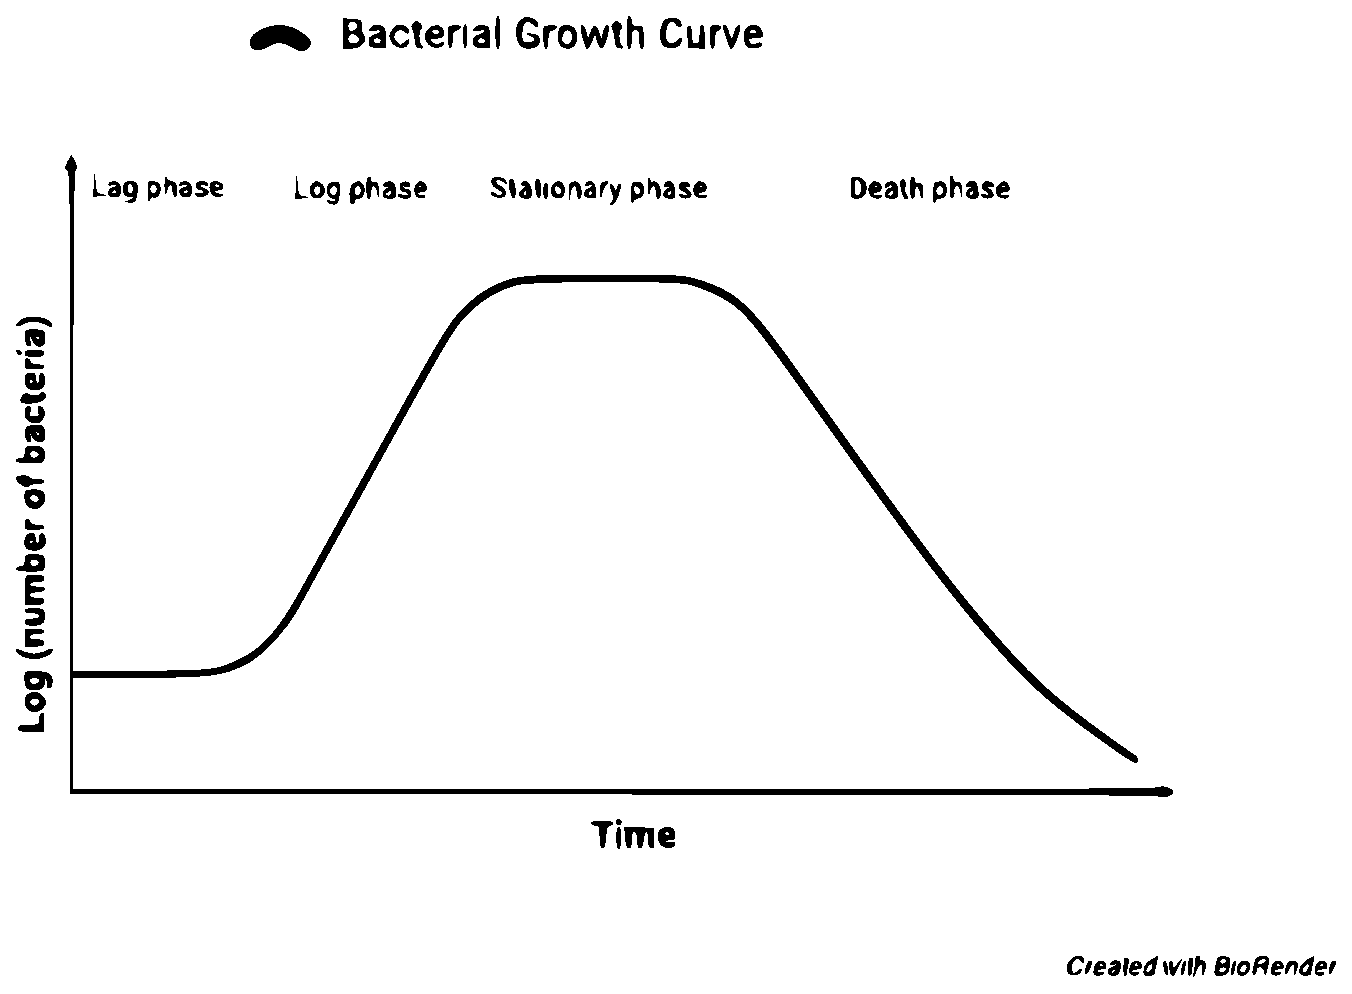
\includegraphics[scale=0.3]{BE21B040/BacterialGrowthGraph.eps}
		}
	\end{center}
	
\end{enumerate} 
\textbf{\Large{Calculation of Generation time}} \\

Generation time is the time taken by the bacteria to double in number as in the previous generation or in simpler terms undergo one binary fission. Common examples such as E. coli have a generation time of 17 minutes in a medium of glucose-salts.

\begin{table}[h]
	\begin{center}
\begin{tabular}{|c|l|}
\hline
	Variables & Description \\
\hline
	$N_0$ & Initial number of bacteria \\
	$N$ & Final number of bacteria \\
	$G$ & Generation time \\
	$n$ & Number of generations \\
	$t$ & Total time period \\
\hline
\end{tabular}
	\caption{Table of variables used in the equation}
	\label{tab:varTimeTable}
	\end{center}
\end{table}

	\[{N} = {N_0}\times{2^n}\]
	Solving for n:
	\[\log{N} = \log{N_0}+{n}\log{2}\]
	\[{n} = \frac{\log{N}-\log{N_0}}{log{2}}\]
    \[{n} = \frac{\log{N}-\log{N_0}}{0.301}\]
    \[{n} = {3.3}\log({\frac{N}{N_0}})\]
    Using eq \ref{eqn:generationTime},
    \[{G} = \frac{t}{n}\]
    \begin{equation}
        {G} = \frac{t}{{3.3}\log({\frac{N}{N_0}})}
    \end{equation}
    
    
\nocite{*}
\bibliography{biblio}
\bibliographystyle{alpha}

\section{CE19B020}
Student shall edit this file and include stuff for the assignment

\section{CE21B021}
Student shall edit this file and include stuff for the assignment

\section{CE21B088}
\begin{center}
    \title{\textbf{\underline{{\huge Planck's Equation}}}}\\[\baselineskip]
    \date{July, 2022} \\[\baselineskip]
\end{center}
\maketitle


\textsf{{\large Planck's law describes the spectral density of electromagnetic radiation emitted by a black body in thermal equilibrium at a given temperature T, where there is no net flow of matter or energy between the body and its environment.}} \\[\baselineskip]
\textsf{{\large This formula is considered one of the most important physics formulas, as it is responsible for the birth of quantum mechanics, also television and solar cells.  Max Planck postulated in 1900, that energy was quantised and could be emitted or absorbed only in integral multiples of a small unit, which he called \textbf{energy quantum}.}}

{\LARGE \[\boxed{ E=hv }\]}
\textsf{\large Alternatively, this equation can be written as : }
{\LARGE \[\boxed{E=hc/\lambda}\]} \\
\textsf{\large This relation gives the energy of a photon E, known as \textbf{photon energy}. This relation states that the photon energy is \textbf{directly proportional to its frequency, \textit{v}.} }
\begin{table}[h!]
   \begin{center}
    \caption{Terms used}
        \begin{tabular}{| c | c |}
       
        \hline
            \textsf{\textbf{TERM}} & \textsf{\textbf{DESCRIPTION}}  \\\hline
            \textsf{E} & \textsf{Energy}  \\\hline
            \textsf{h} & \textsf{Planck's constant, whose value is $6.62607015$ × $10^{-34} m^2 kg / s$}  \\\hline
            \textsf{\textit{v}} & \textsf{Frequency of the incident light} \\ \hline
            \textsf{c} & \textsf{Speed of light, whose value is 299,792,458 m/s} \\ \hline
            $\lambda$ & \textsf{Wavelength of the incident light} \\ \hline
        \end{tabular}
    \end{center}
    \end{table}
    \\[2\baselineskip]
    \\[2\baselineskip]
    \begin{center}
        {\Large ---Thank You---}
    \end{center}


\section{CE21B097}
\begin{equation}
    \boxed{e^{\iota\pi}+1=0}
\end{equation}
\\The equation above is called "\textbf{Euler's identity}". It is named after the Swiss mathematician \textbf{Leonhard Euler}. It's a special case of Euler's formula which is\quad$e^{\iota x}= \cos{x} + \iota\sin{x}$\quad when x = $\pi$. Euler's identity is often cited as an example of deep \textbf{mathematical beauty}. This is because it connects the most fundmental numbers in mathematics e, $\pi$, $\iota$ in a very simple manner. \\ \\ \\ \\ \\ \\
\begin{center} \includegraphics[width=0.20\textwidth,natwidth=610,natheight=642]{euler.eps}
\end{center}
The figure above signifies the value of\quad$e^{\iota x}= \cos{x} + \iota\sin{x}$\quad based on $\phi$ plotted on the Real, Imaginary number plane.  
\begin{table}[htbp]
\centering
\begin{tabular}{|l|p{0.8\linewidth}|}
\hline
\multicolumn{1}{|c|}{\textit{\textbf{Symbols}}} & \multicolumn{1}{c|}{\textit{\textbf{Explanation}}}                                                   \tabularnewline \hline
$\pi$                                              &    The number $\pi$ is a mathematical constant that is the ratio of a circle's circumference to its diameter, approximately equal to 3.14159.                                            \tabularnewline \hline
$\iota$                                             &   Complex Numbers in Maths. Complex numbers are the numbers that are expressed in the form of a+ib where, a,b are real numbers and 'i' is an imaginary number called “iota”. The value of i = ($\sqrt{-1}$).                                                                            \tabularnewline \hline
e                                           &        The number e, also known as Euler's number, is a mathematical constant approximately equal to 2.71828 which can be characterized in many ways. It is the base of the natural logarithms. It is the limit of (1 + 1/n)n as n approaches infinity                                                        \tabularnewline \hline
\end{tabular}
\end{table}

\section{CE21B112}
Student shall edit this file and include stuff for the assignment


\section{CE21B115}


\title{\textbf{Assignment 4}}
\author{\textbf{Sankar M, CE21B115 }}
\date{\textbf{June 2022}}

\maketitle
\subsection{Maxwell's equation}

\begin{equation}
   \Vec{\nabla}\cdot\Vec{E} = \frac{\rho}{\epsilon_{0}} 
\end{equation}

\begin{equation}
   \Vec{\nabla}\cdot\Vec{B} = 0 
\end{equation} 

\begin{equation}
    \Vec{\nabla}\times\Vec{E} = -\frac{\partial\Vec{B}}{\partial t} 
\end{equation}

\begin{equation}
    \Vec{\nabla}\times\Vec{B}=\mu_{0} (\Vec{J} + \epsilon_{0} \frac{\partial\Vec{E}}{\partial t} )
\end{equation}

\begin{center}
\begin{tabular}{|c|c|}
    \hline
    \textbf{Symbols} & \textbf{Explanation} \\
    \hline
    $\mu_{0}$ & permeability of free space \\
    \hline
    $\epsilon_{0}$ & permittivity of free space \\
    \hline
    $\rho$ & electric charge density, charge per unit volume \\
    \hline
    $\Vec{J}$ & free current density, current per unit area  \\
    \hline
    $\Vec{E}$ & Electric Field \\
    \hline
    $\Vec{B}$ & Magnetic Field \\
    \hline
\end{tabular}
\end{center}

\begin{center}
    \begin{tabular}{|c|c|}
    \hline
    $\nabla$  & denotes the gradient operator, del  \\
    \hline
    $\nabla\cdot$ & denotes the divergence operator \\
    \hline
    $\nabla\times$ & denotes the curl operator \\
    \hline
    \end{tabular}
\end{center}


Ampere stated the relation between magnetic field and electric current. Maxwell added that magnetic field can also be related to changing electric field which he called as displacement current, $\Vec{J_{d}}=\epsilon_{0} \frac{\partial\Vec{E}}{\partial t}$.As a result of Maxwell's addition, ampere's
law was true even when it is not a static condition.

Maxwell's equation highlights the fact how the divergence and curl of electric and magnetic fields are related. They say that the electric fields can be produced by charges($\rho$) or by changing magnetic fields($\frac{\partial\Vec{B}}{\partial t}$). And magnetic  fields can be produced either by currents($\Vec{J}$) or by changing electric fields($\frac{\partial\Vec{E}}{\partial t}$) 



% \section{CH21B067}


% \documentclass{article}
% \usepackage[utf8]{inputenc}
% \usepackage{hyperref}

\title{Schrödinger's Equation}
\author{Nishanth Nethaniel Magesh ch21b067}
\date{June 2022}

% \begin{document}

\maketitle

\section{Description}

Schrödinger's Equation is considered to be one of the essential equations in quantum mechanics. Its role is similar to that of Newton's Laws and Conservation of Energy in Classical Mechanics i.e. predicting the future behaviour of a quantum mechanical system. The solution of this equation gives the wavefunction $\psi$, which can be used to find the probability of the existence of a particle at each point of the system.

\section{Equation}

\begin{equation}
    i\hbar\frac{\partial}{\partial t}\psi=[-\frac{\hbar^2}{2m}\nabla^2+V]\psi
\end{equation}

The operators on the left and right sides are often reduced to $\hat{H}$  and $\hat{E}$ respectively for convenience:

\begin{equation}
    \hat{E}\psi=\hat{H}\psi
\end{equation}

i.e.$$ \hat{E}=i\hbar\frac{\partial}{\partial t} \:\:\:and\:\:\:\hat{H}= -\frac{\hbar^2}{2m} \nabla^2+V $$

\begin{table}
    \begin{center}
    \begin{tabular}{|c|c|}
    \hline
        i & Imaginary unit($\sqrt{-1}$) \\
    \hline
        $\hbar$ & Reduced Planck's constant \\
    \hline    
        m & mass \\
    \hline    
        V & Potential field \\
    \hline    
        $\psi$ & Wave Function \\
    \hline    
        $\hat{E}$ & Energy Operator \\
    \hline    
        $\hat{H}$ & Hamiltonian Operator \\
    \hline
    \end{tabular}
\end{center}
    \caption{Explanation of terms used}
\end{table}


\section{Explanation}

The equation above is more specifically called the time-dependant Schrödinger's equation. It is used to find the evolution of the wavefunction $\psi$ over time. $\hat{H}$ is known as the Hamiltonian Operator, which corresponds to the total energy of the system. It consists of 2 terms:

\begin{itemize}
    \item -$ \frac{\hbar^2}{2m}\nabla^2 $ - This term is the kinetic energy operator. As the name suggests, it gives the kinetic energy for the wavefunction it operates on
    \item V - The potential energy function describes the potential energy of the particle
\end{itemize}

The term $\hat{E}$ is the Total Energy operator. In the simpler time-independent Schrödinger's
 equation, it is represented as E (without the hat). E is the eigenvalue of the Hamiltonian operator acting on $\psi$

\begin{equation}
    E\psi=\hat{H}\psi
\end{equation}

This equation describes quantum stationary states, whose properties don't depend on time i.e. are constant.

\end{document}

\section{CH21B079}
Student shall edit this file and include stuff for the assignment

\section{CH21B101}

\documentclass{report}
\usepackage[utf8]{inputenc}
\usepackage{geometry}
 \geometry{
 a4paper,
 total={170mm,257mm},
 left=20mm,
 top=20mm,
 }

\begin{document}
\Large{\textbf{Roll NO. CH21B101}}
\newline
\newline
\huge{\textit{\underline{UNIVERSAL LAW OF GRAVITATION}}}
 
\section{Overview and Definition}
\Large{
\Large Universal law of Gravitation was coined by sir Issac Newton as an attractive force between two masses in a space.
\newline
\newline
\textbf{\textit{UNIVERSAL LAW OF GRAVITATION:}} \Large When considered two masses in a space with masses $m_1$ and $m_2$ respectively then the attractive force between them is directly proportional to the product of their masses [$m_1*m_2$] and inversely proportional to the square to the square of distance between them.
}
\section{Formulation}
 
\large{$F= G(m_1*m_2)/r^2$}
\huge{ 
\begin{center}
\begin{tabular}{ |c|c| } 
 \hline
 $G$ & Universal Gravitation Constant \\
 $r$ & Distance between $m_1$ and $m_2$ \\
 $m_1$ & Mass of body 1 \\
 $m_2$ & Mass of body 2 \\
 F & Force between the two bodies \\
 \hline
\end{tabular}
\end{center}
}
\section{Properties}
\begin{itemize}
\Large{
 \item It acts along the line joining the two masses.
 \item It is an attractive force with smaller magnitude compared to other forces like nuclear forces or electrostatic forces.
 \item It is an inverse square law which means the intensity of force inversely depends upon the square of the distance between the two masses.
} 
\end{itemize} 

\end{document}

\section{ME21B050}
Student shall edit this file and include stuff for the assignment

\section{ME21B060}
Student shall edit this file and include stuff for the assignment

\section{ME21B065}
Student shall edit this file and include stuff for the assignment

\documentclass{article}

\usepackage[utf8]{inputenc}
\usepackage{graphicx}
\usepackage{array}
\title{Assignment 4}
\author{jayaram hemachander.}
\date{June 2022}

\begin{document}

\maketitle
\section{Maxwell Equation}
\begin{figure}[h]
\centering\includegraphics[width=0.5\textwidth]{maxwell}
\end{figure}
Faraday's law
$$ \frac{\partial\mathcal{D}}{\partial t} \quad  = \quad \nabla\times\mathcal{H}$$
Ampère's Law
$$ \frac{\partial\mathcal{B}}{\partial t} \quad  = \quad -\nabla\times\mathcal{E}$$
Gauss Law
$$ \nabla\cdot\mathcal{B}\quad  = \quad 0, \quad$$
Colomb's Law
$$ nabla\cdot\mathcal{D}\quad  = \quad \rho_{v} ,$$

\subsection{Faraday's Law}
When the magnetic flux linking a circuit changes, an electromotive force is induced in the circuit proportional to the rate of change of the flux linkage.
\subsection{Ampère's Law}
The magnetic field created by an electric current is proportional to the size of that electric current with a constant of proportionality equal to the permeability of free space
\subsection{Gauss Law}
Gauss's law for magnetism states that the magnetic flux B across any closed surface is zero
\subsection{Colomb's Law}
The closed line integral of magnetic field vector is always equal to the total amount of scalar electric field enclosed within the path of any shape
\section{Expansion of variables}



\begin{center}
\begin{tabular}{ | m{5cm} | m{5cm} | } 
  \hline
  \textbf{Symbol} & \textbf{Expansion}  \\ 
  \hline
  $$\mathcal{D}$$ & The volume of electric charge density \\ 
  \hline
  $$\mathcal{B}$$ & The magnetic field \\  
  \hline
  $$\mathcal{E}$$ & The electric field \\  
  \hline
  $$\mathcal{H}$$ & Magnetic field strength \\  
  \hline
  $$\rho_{v}$$ & Free Charge Density\\
  \hline
\end{tabular}
\end{center}
\end{document}

\section{ME21B088}
Student shall edit this file and include stuff for the assignment

\section{ME21B091}
Student shall edit this file and include stuff for the assignment

\section{ME21B186}
Student shall edit this file and include stuff for the assignment

\documentclass{article}
\usepackage[letterpaper,top=2cm,bottom=2cm,left=3cm,right=3cm,marginparwidth=1.75cm]{geometry}
\usepackage{amsmath}
\usepackage{graphicx}

\begin{document}
\title{\textbf{\huge{Ampere's Law}}}
\author{ID2090 Assignment 4\\
Ronalyn Sequeira : ME21B186}
\maketitle

\begin{flushleft}
\large{Ampere's law can be written as the curl of B as :} \\
\end{flushleft}
\begin{center}
\boldmath
\large{$ $$\nabla$$ \times \vec{B} = {\mu_0}\vec{J}$} \\
\unboldmath
\end{center}

\large{\begin{tabular}{|c|c|}
\hline
 B  &  Magnetic field \\
 \hline
${\mu_0}$ & Permeability of free space\\
\hline
${\vec{J}}$ & Current density \\
\hline
\end{tabular}}\\
\\
\\
\large{The integral form of the Ampere's Law comes from the Stokes' theorem, which can be given as}
\begin{center}
\boldmath
\large{$$\oint{\vec{B}} \cdot d{\vec{l}} = {\mu_0}{\vec{I}_{enc}}$$}
\unboldmath
\end{center}

\begin{figure}[!ht]
    \centering
    \includegraphics[width=0.3\textwidth]{id_1.png}
    \caption{Current carrying loop}
    \label{fig:my_label}
\end{figure}

\large{$\oint{\vec{B}} \cdot d{\vec{l}}$ \text{is the line integral of the magnetic field around a closed current carrying loop.}
\large{$\vec{I}_{enc}$ \text{is the amount of current passing through the loop.}\\



\large{The equation helps in calculating the magnetic field around a current carrying closed loop.It even helps in calculating the current enclosed in a closed loop when the magnetic field is known.\\

The equation is known more for its application to symmetric systems.To find the magnetic field along a circular loop, around a cylinder carrying current axially, etc Ampere's law is very helpful and mak>
}

\end{document}

\section{ME21B190}
\subsection{Navier-stokes equation}
   
\begin{figure}[h]
\centering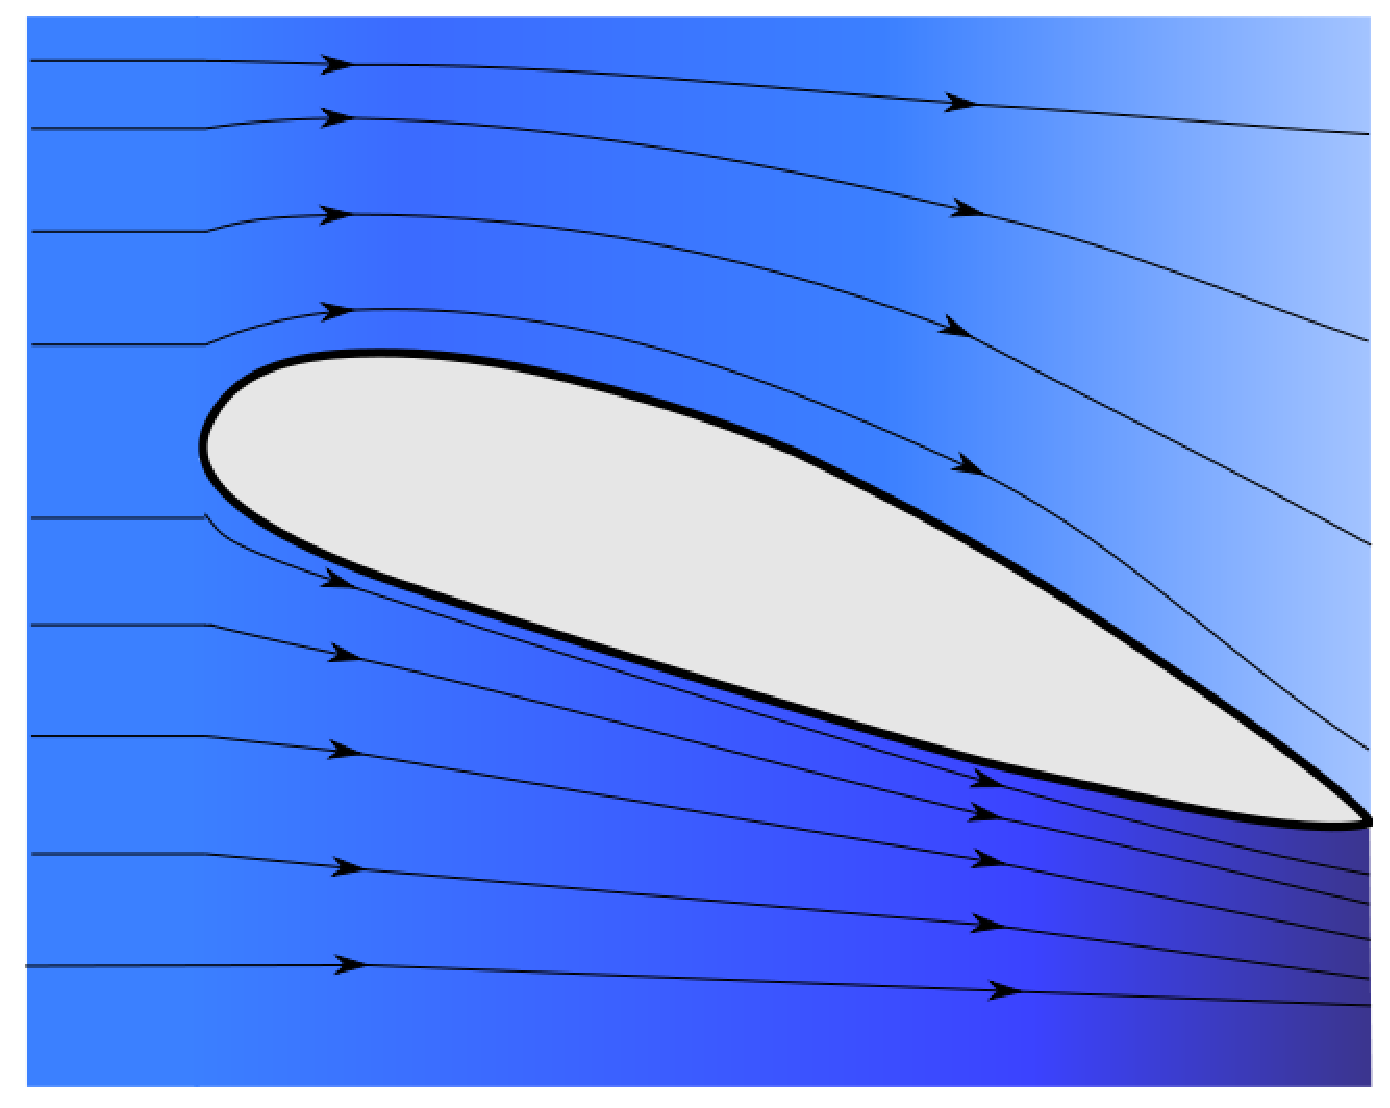
\includegraphics[width=0.5\textwidth]{./ME21B190/air.eps}
\end{figure}
\subsection{Continuity Equation:}

$$\nabla.\vec{V}=0$$


\large\ The countinuity equation describes the trasport of some quantities like fluid or gas.The equation explains how a fluid conserves mass in its motion.
\subsubsection {Momentum Equations:}

$$\frac{d\vec{V}}{dt}=\frac{\partial V}{\partial t} + (V.\nabla)V$$
\ Here the total derivative is the sum of change in velocity with time and the convective term
$$\rho\frac{d\vec{V}}{dt}=-\nabla{p} + \rho\vec{g}+\mu\nabla^{2}\vec{V}$$
 *The first term in RHS is the "Pressure gradient term" which tells in which direction the fluid flows

*The second term is the "Body force term",which includes all type of forces
*The third term "Diffusion term" 
\subsection{Explanation of variables}
\begin{center}
\begin{tabular}{ c c } 
   \hline
   \textbf{Symbol} & \textbf{Explanation} \\
   \hline
   $\vec{V}$ & velocity vector \\
   \hline
   $\rho$ & density of fluid \\
   \hline
   $\vec{g}$ & acceleration due to gravity \\
   \hline
   ${p}$ & pressure of fluid \\
   \hline
   $\mu$ & viscosity of fluid \\
   \hline
\end{tabular}
\end{center}

\section{ME21B196}

\subsection{Thermodynamics of a Control Volume}

Calculations of thermodynamic variables in a "control volume" (i.e., a system that has a constant volume but might have varying mass and energy contained in it) involve the equation of energy conservation as follows:
$$\dot{Q} - \dot{W} = \dfrac{dE}{dt} + \dot{m_e}(h_e + gz_e + \dfrac{1}{2}v_e^2) - \dot{m_i}(h_i + gz_i + \dfrac{1}{2}v_i^2)$$~\cite{cvpsu}.~\cite{cvsfu}.

Here the $i$ and $e$ subscripts denote inlet and exit values, respectively.

\begin{figure}[h]

	\begin{center}
		\framebox{
			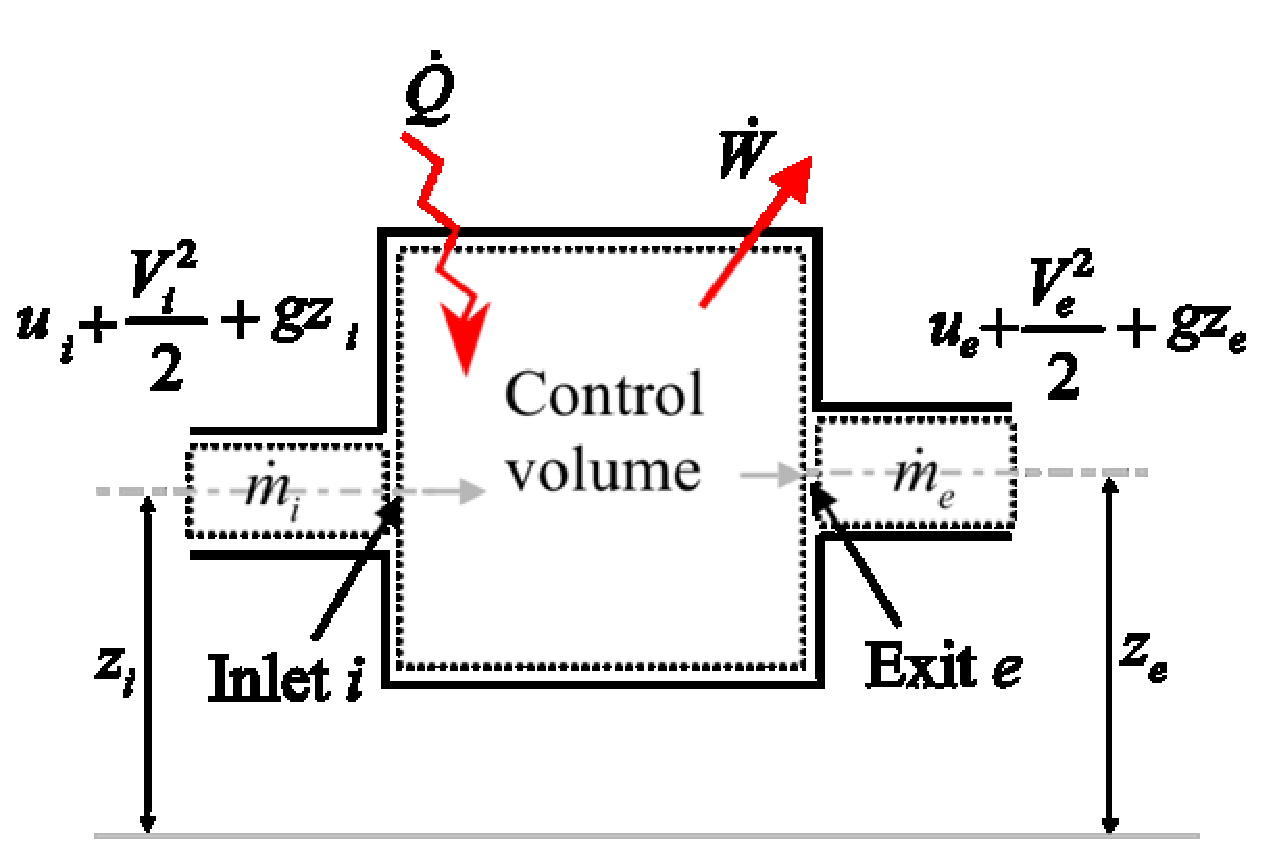
\includegraphics[scale=0.5]{ME21B196/CV.eps}
			}
	\end{center}
	
	\caption{The diagram of a control volume. Credits: \href{https://www.chegg.com/homework-help/fundamentals-of-engineering-thermodynamics-8th-edition-chapter-4-problem-1e-solution-9781118412930}{Chegg.com}.}

	\label{CV}
\end{figure}

\begin{table}[h!]

\begin{center}

	\caption{Key of symbols}
	
	\begin{tabular}{|c|r|l|}

\hline
	Sl No. & Symbol & Explanation \\
	\hline
	1 & $Q$ & Heat interaction of the system \\
	2 & $W$ & Work interaction of the system \\
	3 & $E$ & Total energy of the system \\
	4 & $t$ & Time \\
	5 & $m$ & Mass \\
	6 & $h$ & Specific enthalpy \\
	7 & $g$ & Acceleration due to gravity \\
	8 & $z$ & Height from a reference height \\
	9 & $v$ & Velocity \\
	\hline

\end{tabular}

\end{center}

\end{table}
\section{ME21B204}
Student shall edit this file and include stuff for the assignment

\section{ME21B217}
Student shall edit this file and include stuff for the assignment

\section{MM21B012}

\title{Bernoulli's Equation}
\author{MM21B012}
\date{July, 2022}

\maketitle				

\subsection{Bernoulli's equation for in-compressible flow}

\begin{equation} 
\Psi = \frac{1}{2} \rho v^2 + \rho gz + p
\end{equation}

\begin{tabular}{|c|l|}
\hline
    Symbol & Description \\
\hline
    v & v is the flow speed at a point on the streamline \\
\hline
    g & g is the acceleration due to gravity \\
\hline
    z & z is the elevation of the point above a reference plane, (in the direction \\
    & opposite to acceleration due to gravity) \\
 \hline
    h & h is the pressure at the chosen point \\
\hline 
    $ \rho $ & $ \rho $  is the density of the fluid at all points of the fluid ( as the fluid \\
    & is in-compressible, it will be constant for all points of the the fluid ) \\
\hline
    $ \Psi $ & $ \Psi $ is a constant \\
\hline
\end{tabular}

\subsection{Explanation}
    In fluid dynamics, Bernoulli's principle states that an increase in the speed of a fluid occurs simultaneously with a decrease in static pressure or a decrease in the fluid's potential energy. The principle is named after Daniel Bernoulli who published it in his book Hydrodynamica in 1738. Although Bernoulli deduced that pressure decreases when the flow speed increases, it was Leonhard Euler in 1752 who derived Bernoulli's equation in its usual form. The principle is only applicable for isentropic flows: when the effects of irreversible processes (like turbulence) and non-adiabatic processes (e.g. heat radiation) are small and can be neglected.
    Bernoulli's principle can be derived from the principle of conservation of energy. This states that, in a steady flow, the sum of all forms of energy in a fluid along a streamline is the same at all points on that streamline. This requires that the sum of kinetic energy, potential energy and internal energy remains constant. Thus an increase in the speed of the fluid – implying an increase in its kinetic energy (dynamic pressure) – occurs with a simultaneous decrease in (the sum of) its potential energy (including the static pressure) and internal energy. If the fluid is flowing out of a reservoir, the sum of all forms of energy is the same on all streamlines because in a reservoir the energy per unit volume (the sum of pressure and gravitational potential $ \rho $gh) is the same everywhere.

\section{MM21B024}
\subsection{Lagrangian Operator}
\[\mathcal{L} = \sum_{i=1} ^ {n} \frac{1}{2} m\Dot{q_i}^2 - U(q_1,q_2,q_3,q_4....q_n)\]
\subsection{Euler Lagrangian Equation}
\[\frac{d}{dt} \frac{\partial \mathcal{L}}{\partial \Dot{q_i}} = \frac{\partial \mathcal{L}}{\partial {q_i}}\]

\subsection{Symbols Involved}
\begin{tabular}{|c|c|}
    \hline
    SYMBOL & DEFINITION \\
    \hline
    $q_i$ & generalised coordinate \\\hline
    $\Dot{q_i}$ & generalised coordinate's velocity $\frac{dq_i}{dt}$ \\\hline
    $\mathcal{L}$ & Lagrangian \\\hline
    $\frac{d}{dt}$ & derivative with respect to time  \\ & \\\hline
    $\frac{\partial \mathcal{L}}{\partial q_i}$ & partial derivative of Lagrangian with respect to $q_i$\\ & \\\hline
    $\frac{\partial \mathcal{L}}{{\partial \Dot{q_i}}}$& partial derivative of Lagrangian with respect to $\Dot{q_i}$\\ & \\\hline
   m & mass of object \\\hline
   $U(q_1,q_2,q_3....q_n)$ & Potential energy of the object \\\hline
    \end{tabular}
    \begin{figure}[ht]
        \centering
        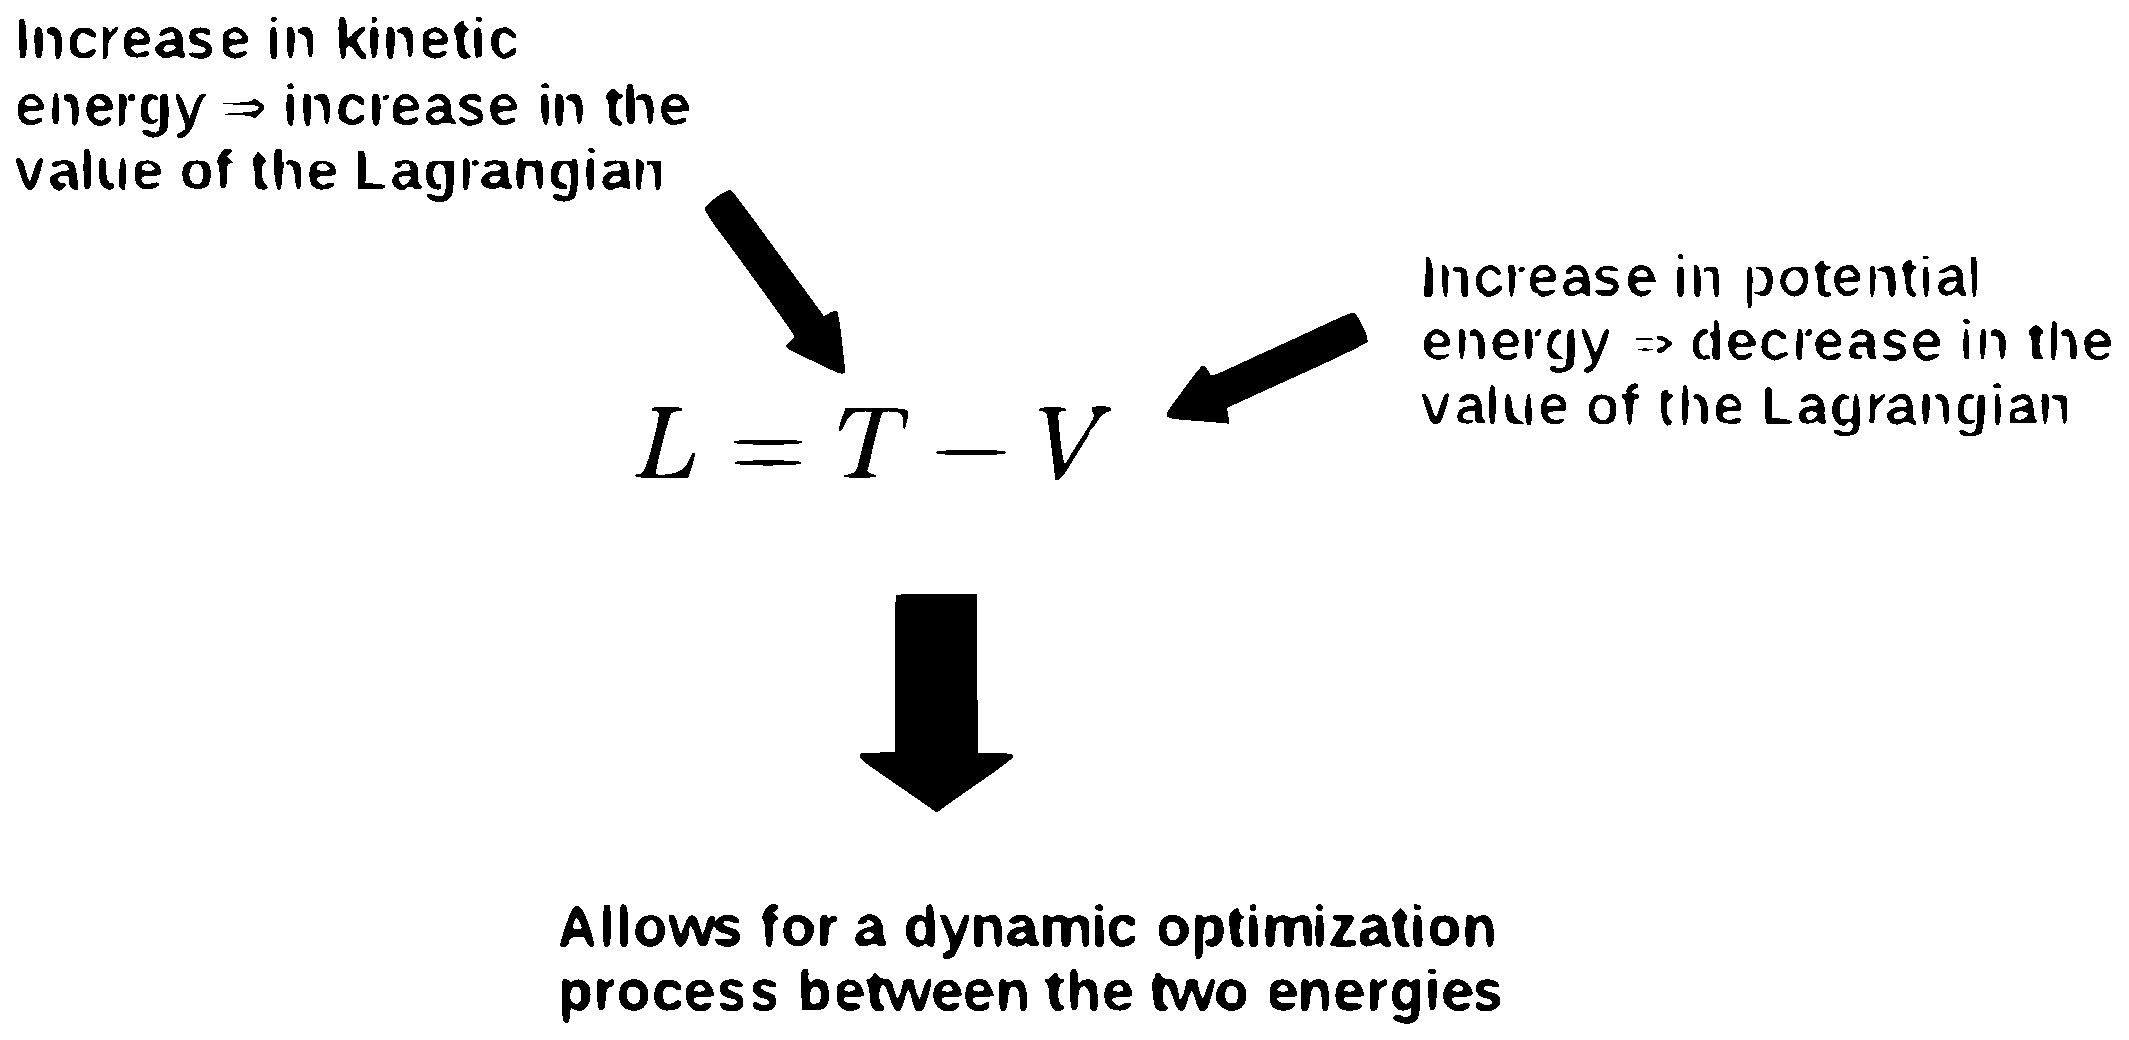
\includegraphics[width=\textwidth]{./MM21B024/image-29.eps}
        \caption{The Lagrangian Operator}
        \label{fig:my_label}
    \end{figure}
    
\section{Explanation of equation}
This is a mechanical model developed by Lagrange to analyse complex systems which are very difficult to analyse by Newtonian Mechanics. The process follows the calculus of variations and defines a procedure to analyse a system by the Euler Lagrangian equation which is a result of Hamilton's principle of least action.The mechanical state of the object i.e its potential and kinetic energies are determined in terms of generalised coordinates. The number of generalised coordinates of a body is same as the number of degrees of freedom it has.The generalised coordinates have their own velocities defined as their derivatives with respect to time. The Lagrangian is now expressed in terms of the generalised coordinates and their velocities. By principle of least action and calculus we arrive at the Euler Lagrangian equation. On proceeding to do the math we get a second order partial differential equation in the generalised coordinate. On solving all the partial differential equations simultaneously we can calculate the exact state of the system at a given time. This setup is generally used to analyse oscillators.  





\section{MM21B032}
Student shall edit this file and include stuff for the assignment

\section{MM21B044}

\subsection{Equation:}
\textbf{Taylor's Series Expansion:}
\begin{multline}
    f(x) \approx f(x_0)+f'(x_0)(x-x_0)+f''(x_0) \frac{(x-x_0)^2}{2!}+...\\
    ...+f^{n'}(x_0) \frac{(x-x_0)^n}{n!}+...  \infty terms
\end{multline}
\[f(x) = \sum_{n=0}^{\infty} f^{(n)}(x_0)\frac{(x-x_0)^n}{n!}\]
\subsection{Description:}
\begin{itemize}
    \item Any function f(x) can be written as a series of its derivatives with respect to x and multiplied by a factor $\frac{(x-x_0)^n}{n!}$.
    \item \underline{Accuracy of expression} is proportional to no of terms evaluated.
    \item Eg.\[e^x \approx 1+x+\frac{x^2}{2!}+\frac{x^3}{3!}+\hdots+\frac{x^n}{n!}+\hdots\]
\end{itemize}
\subsection{Table of Variables:}
\begin{tabular}{|c|c|c|}
     \hline
     \textbf{Variables} & \textbf{Expressions} & \textbf{Explanation} \\ \hline
     $f'(x_0)$ & df/dx & 1st order Derivative of f(x) with respect to x \\ \hline
     $f''(x_0)$ & $d^2f/dx^2$ & 2nd order Derivative of f(x) with respect to x \\ \hline
     \vdots & \vdots & \vdots \\ \hline
     $f^{(n)}(x_0)$ & $d^nf/dx^n$ & nth order Derivative of f(x) with respect to x \\ \hline
\end{tabular}

\section{MM21B046}
Student shall edit this file and include stuff for the assignment

\section{MM21B059}
Student shall edit this file and include stuff for the assignment

\section{MM21B063}
- Student shall edit this file and include stuff for the assignment
+
+ \subsection{Equation:}
+ \textbf{Mass-energy equivalence:}
+ \begin{equation}
+        \text{E} = {mc^2}
+        \lable{eqn:E}
+ \end{equation}
+ \[E = mc^2\]
\subsection{Description:}
\begin{itemize}
    \item In Physics, mass-energy equivalence is the relationship between mass and energy in a system's rest frame.
    \item The principle is described by the physicist Albert Einstein's famous formula: $E = mc^2$.
    \item It is famous because Its association with one of the most devastating weapons produced by Humans - the atomic bomb.
\end{itemize}
\subsection{Table of Variables:}
\begin{tabular}{|c|c|c|}
     \hline
     \textbf{Variables} & \textbf{Meaning} & \textbf{Units} \\ \hline
     $E$ & Energy & Kg(m/s)^2 \\ \hline
     $m$ & Mass & Kg \\ \hline
     $c^2$ & Speed of light(3*10^8) & (m/s^2) \\ \hline
\end{tabular}

\section{NA21B002}
Student shall edit this file and include stuff for the assignment

\section{NA21B005}
Student shall edit this file and include stuff for the assignment

\documentclass{article}
\usepackage[margin=1in]{geometry}


\title{Equations of Motion}
\author{Amol Agrawal NA21B006}
\date{June 2022}

\begin{document}

\maketitle

\section{Basic equations of motion}
Suppose a body moving in a 2-D plane starts it motion with an initial velocity $\bf\vec u = u_x + u_y$ and moves with a constant acceleration of $\bf\vec a= a_x + a_y$. At any time $\bf t$ its velocity $\bf \vec v$ and displacement $\bf \vec S$ can be found using following equations:\\ 
\begin{equation}
    \vec v^2 = \vec u^2 + 2\vec a \vec S
\end{equation}
\begin{equation}
    \vec v = \vec u + \vec a  t
\end{equation}
\begin{equation}
    \vec S = \vec u t + 1/2 \vec a t^2
\end{equation}
\\
All of the above equations are derived using calculus and making appropriate assumptions that acceleration remains constant as $a_x$ and $a_y$ in the x and y direction respectively.
They are commonly known as "equations of motion" as they completely describe the motion of a rigid body.\\ \\
\begin{center}
\begin{tabular}{ |l|l| } 
 \hline
 $\vec u$ & Initial velocity possessed by the object which is resolution-ed into x and y components \\  
 $\vec a$ & Resolution-ed acceleration of the object which is defined as the rate of change of its velocity. \\ & For these equations of motion it is constant assuming that a constant force acts upon it.\\ 
 $\vec S$ & Displacement is defined as the separation between the initial and final positions of the object \\ & irrespective of the path that they followed. Unlike distance covered by the object, it is \\ & a vector quantity.\\ 
 t & Total time taken by the object to complete its journey\\
 \hline
\end{tabular}
\end{center}
\end{document}

\include{NA21B007/NA21B007}
\section{NA21B020}
Student shall edit this file and include stuff for the assignment

\section{NA21B048}
Student shall edit this file and include stuff for the assignment

\section{NA21B052}
Student shall edit this file and include stuff for the assignment


% -------------------------------------------------

\section{Conclusions}

If this master tex file could be compiled successfully, it means that the class has learnt the concepts of Git as well as LaTeX properly.

\section{References}
\bibliography{refs}
\bibliographystyle{plain}

\end{document}
